\section{Experimental Results}
\label{sec:experiment}
This section discusses the application of our approach for detecting group anomalies. We begin by briefly describing the dataset used for our experiments in Section~\ref{sec:data_collection} and then move on to discussing the implementation details of how the graph $\mathbf{G}$ is assembled; we construct the graph wavelets $\psi_{s,a}$ in Section~\ref{sec:experimental_setup}. The following section presents the group anomaly detection performance for identifying protest events. In Section~\ref{sec:highlighted_results}, we describe three case studies that illustrate how the graph wavelet model is able to capture absenteeism events such as disaster scenarios.

\begin{figure}[t]
	\centering
	\subfigure[]{
		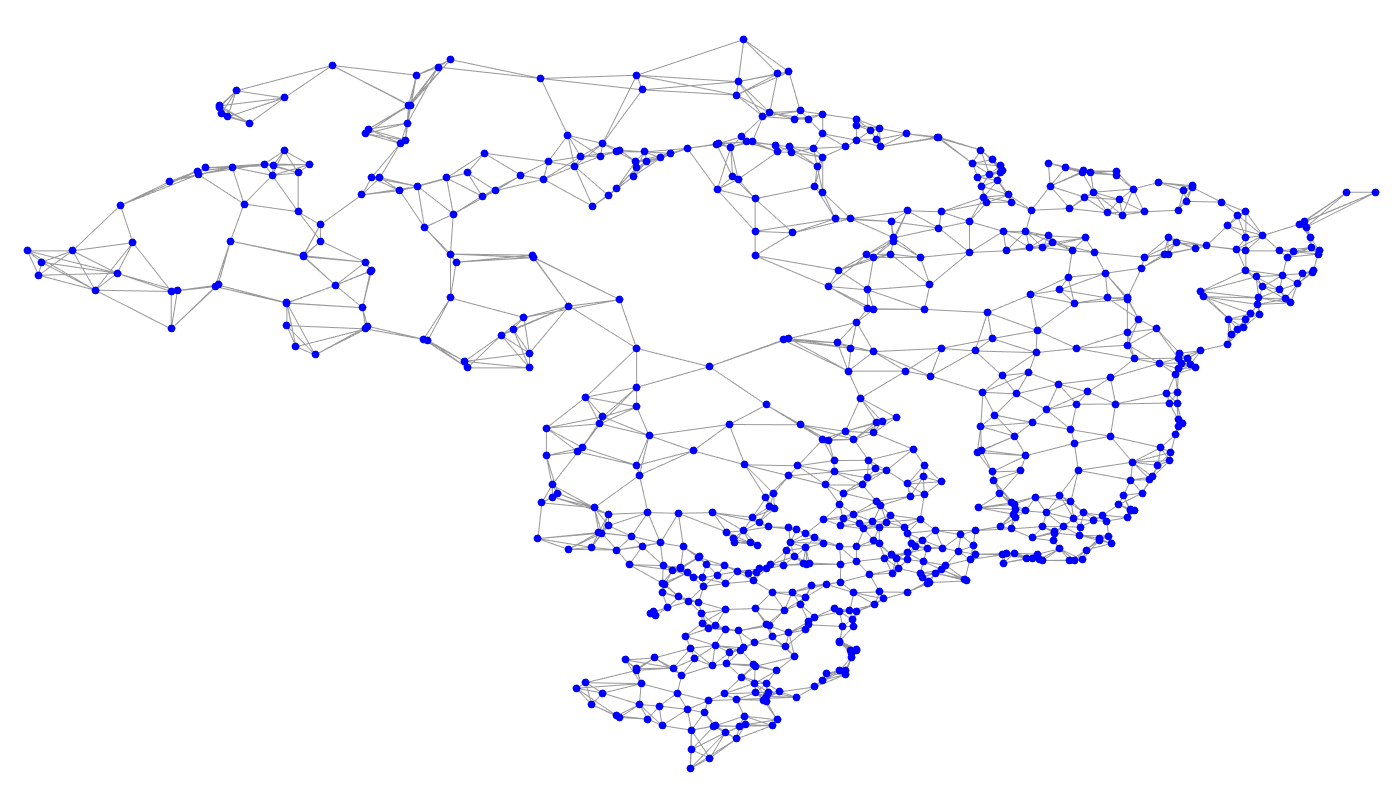
\includegraphics[width=2.8in,height=2.6in] {figures/brazil_graph_nn_5.png}
		\label{fig:brazil_graph_nn_5}
	}
	\subfigure[]{
		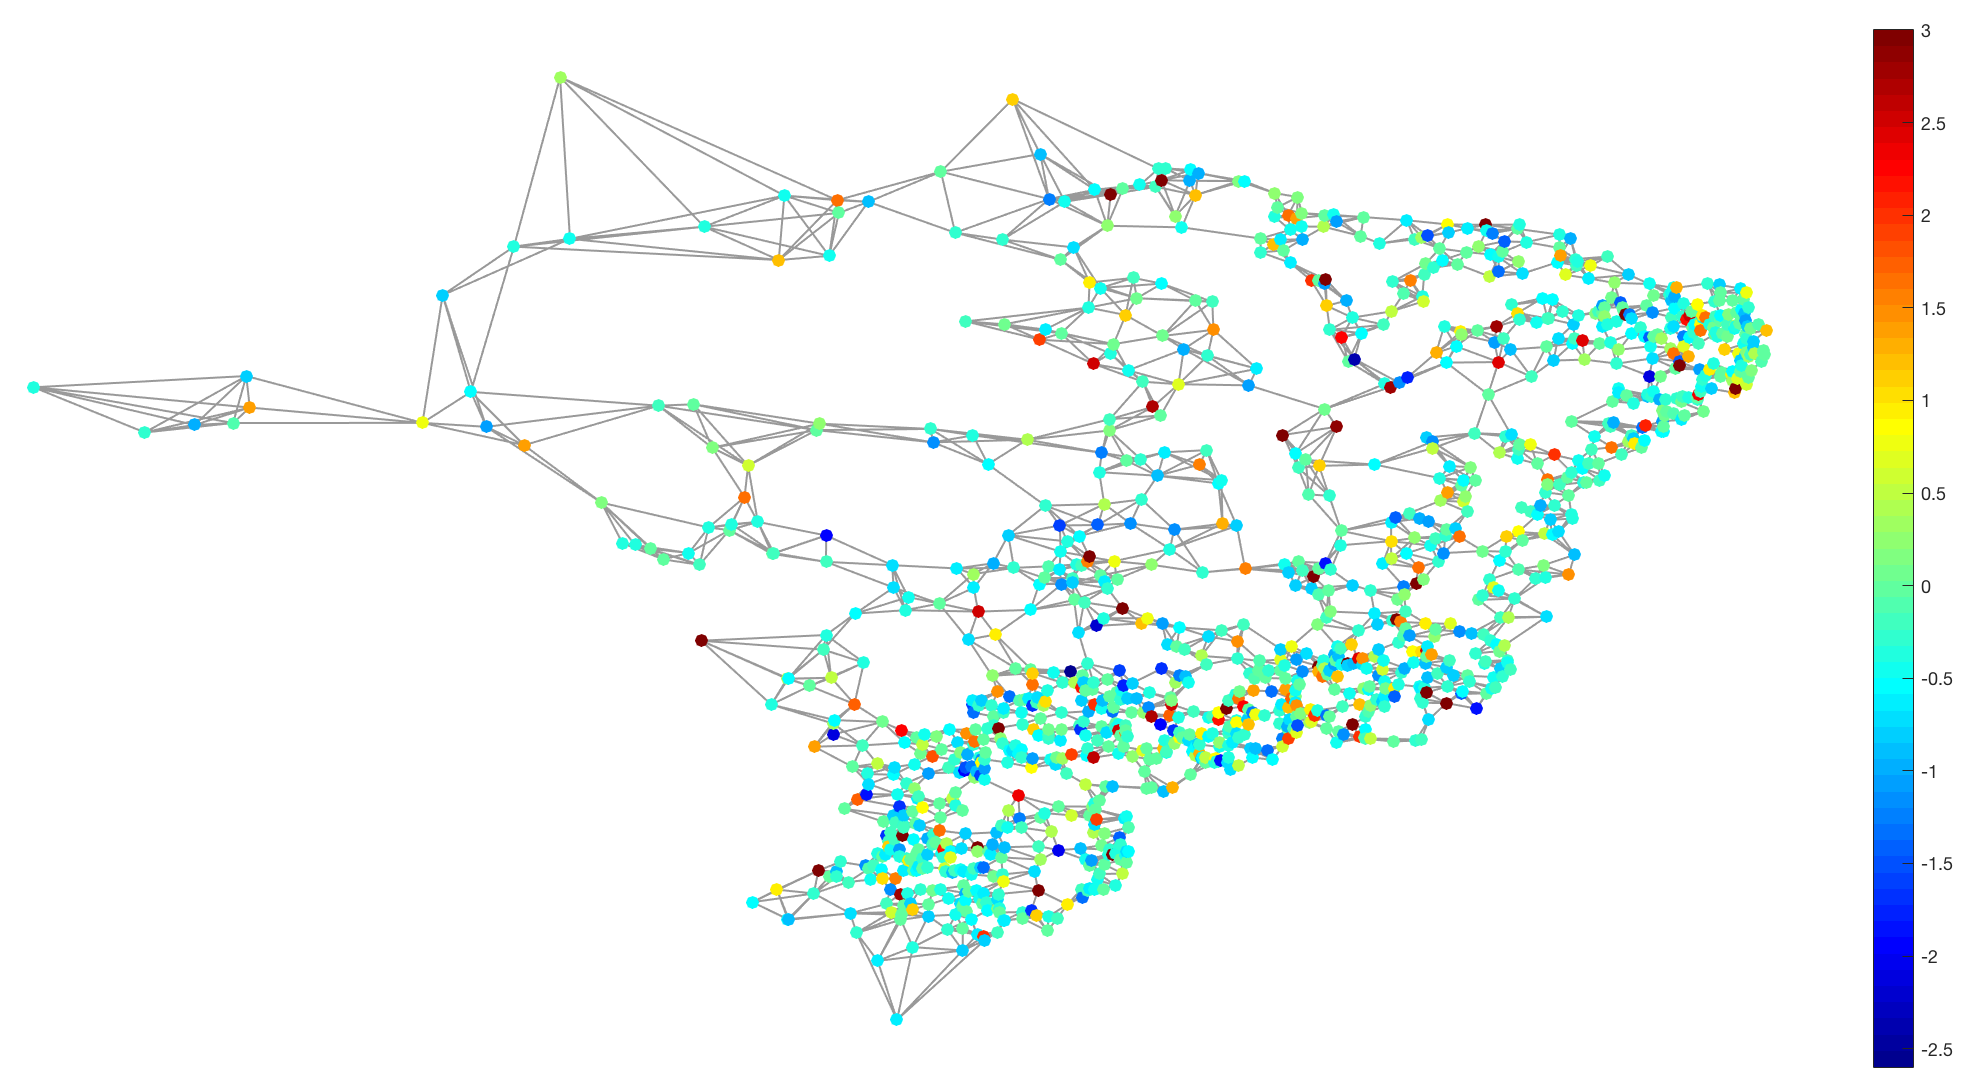
\includegraphics[width=2.8in,height=2.6in] {figures/brazil_zscore_31.png}
		\label{fig:brazil_zscore_31}
	}
	\caption{(a) Brazil's 5-nearest-neighbor graph: 5321 cities, where all edges' weights are $1$. (b) Brazil's z-score distribution on July 31, 2013. The color bar shows the scale of z-score.}
	\label{fig:knn_zscore}
\end{figure}


\subsection{Data Collection and Preprocessing}
\label{sec:data_collection}
The study described in this chapter uses tweets geolocated to Latin America and
collected over a period of two years
(Jan 2013 to Dec 2014).
We query Datasift's streaming API to collect tweets that also have meta-information including geotag bounding boxes (structured geographical coordinates), Twitter places (structured data), user profile location (unstructured, unverified strings), and `mentions information' about locations present in the body of the tweet.
Typically, we found that
the number of tweets with readily available geo-coordinates is too low for conducting meaningful experiments.
To circumvent this drawback, we use the geo-enrichment algorithm described in~\cite{ramakrishnan2014beating}.
This algorithm uses a gazetteer-based approach to look-up location names and geo-coordinates.
To identify location-specific tweets, we configure the geocoding tool to first consider the tweet's text for mentions of place names and geographical landmarks (e.g., say, Plaza de la Independencia (Quito, Ecuador)).
In cases when no geographical location was found in the tweet text, it then proceeds to process the geographical coordinates and the self-reported location string in user's profile metadata.


%To prepare a dataset of ground truth events for our study, we focused on specific types of disruptive societal events, such as natural disasters.
%We assume that such events are the predominant reasons that can cause group absenteeism on social networks.
%To discern when major events occurred, we retrieved records of natural disaster related events involving earthquakes, floods, and landslides from European Emergency Response Coordination Center(ERCC)~\footnote{http://erccportal.jrc.ec.europa.eu/} and World Top Stories Timeline~\footnote{http://www.mapreport.com/}.



\subsection{Experimental Setup}
\label{sec:experimental_setup}

\paragraph{Graph Setup}
Each city $v_i$'s location is represented by its geographical coordinate pair $lat_i$ and $lon_i$. Instead of using the real physical distance, we define the distance of any two cities $v_i$ and $v_j$ as $d_{ij}=\sqrt{(lat_i-lat_j)^2+(lon_i-lon_j)^2}$. We setup graph $G$ as a $k$ neighbors graph, which means  each city is only  connected to its $k$-nearest-neighbors. In this chapter, we set $k=5$, and all the edges' weights  in $G$ are 1. Figure~\ref{fig:brazil_graph_nn_5} shows Brazil's $5$ nearest-neighbor graph with 5321 cities.

\begin{figure}[t]
	\centering
    {
		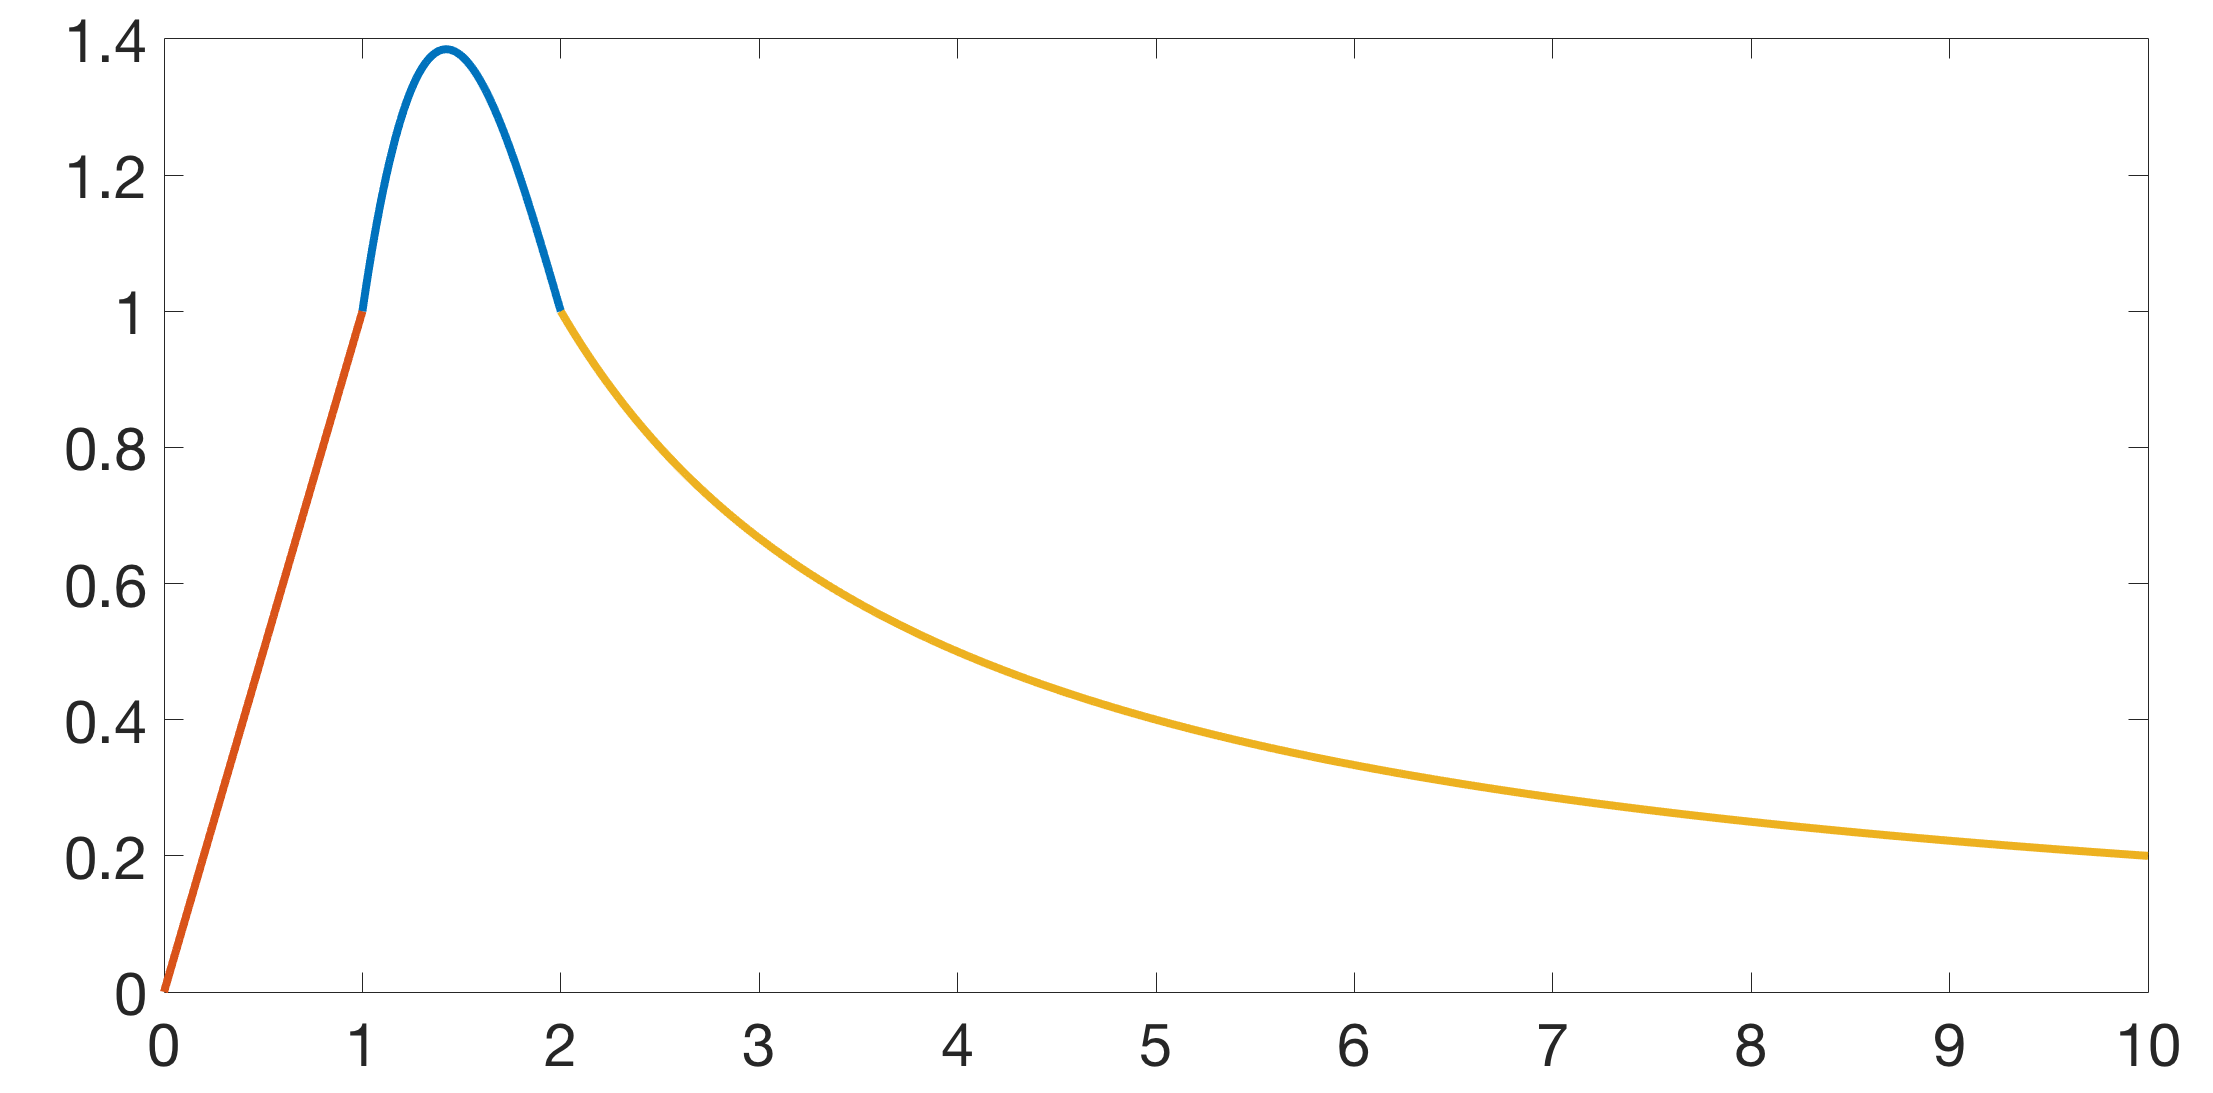
\includegraphics[width= 4in] {figures/kernel_function.png}
		\label{fig:kernel_function}
	}
	\caption{Kernel function g(x).}
	\label{fig:kernel_function}
\end{figure}


\paragraph{Absenteeism Score}
Considering that
the tweet volume $X$ varies vastly among cities, instead of using $X$ itself, we use the normalized value of z-score as absenteeism score, which is defined as:
\begin{equation}
\label{eq:Z_score}
\textrm{z-score} = \frac{X-\mu}{\sigma}
\end{equation}where $\mu$ is the mean value of the previous $30$ day tweets volume and $\sigma$ is the corresponding standard deviation. As shown in Figure~\ref{fig:brazil_zscore_31}, different
node colors denote different z-score values.



\begin{figure}[t]
	\centering
	\subfigure[wavelet $\psi_{s_1,a}$]{
		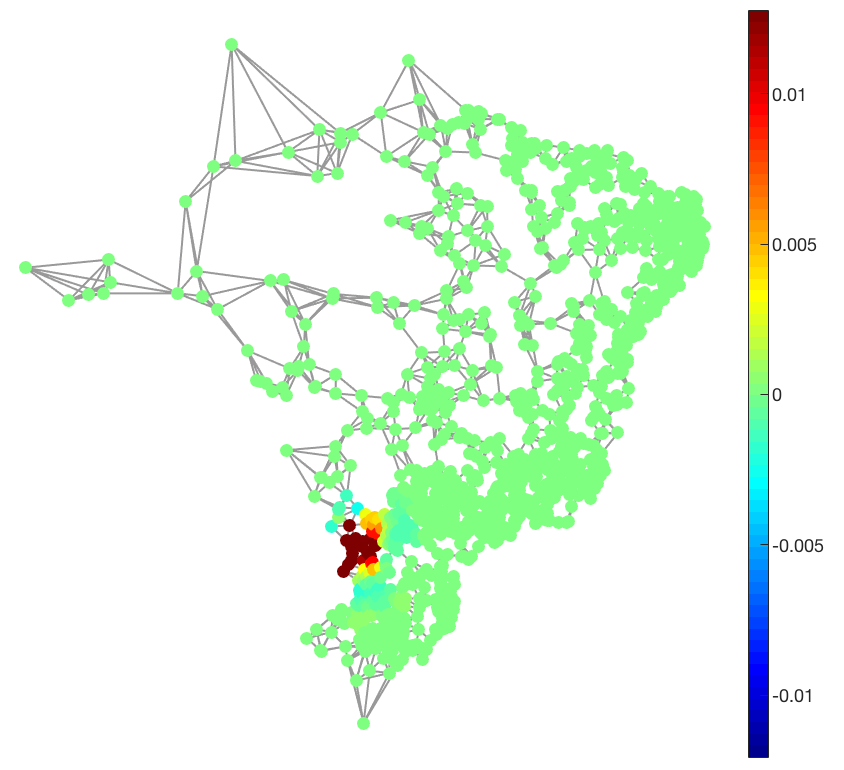
\includegraphics[width=2.8in] {figures/s1.png}
		\label{fig:Brazil_s1}
	}
	\subfigure[wavelet $\psi_{s_2,a}$]{
		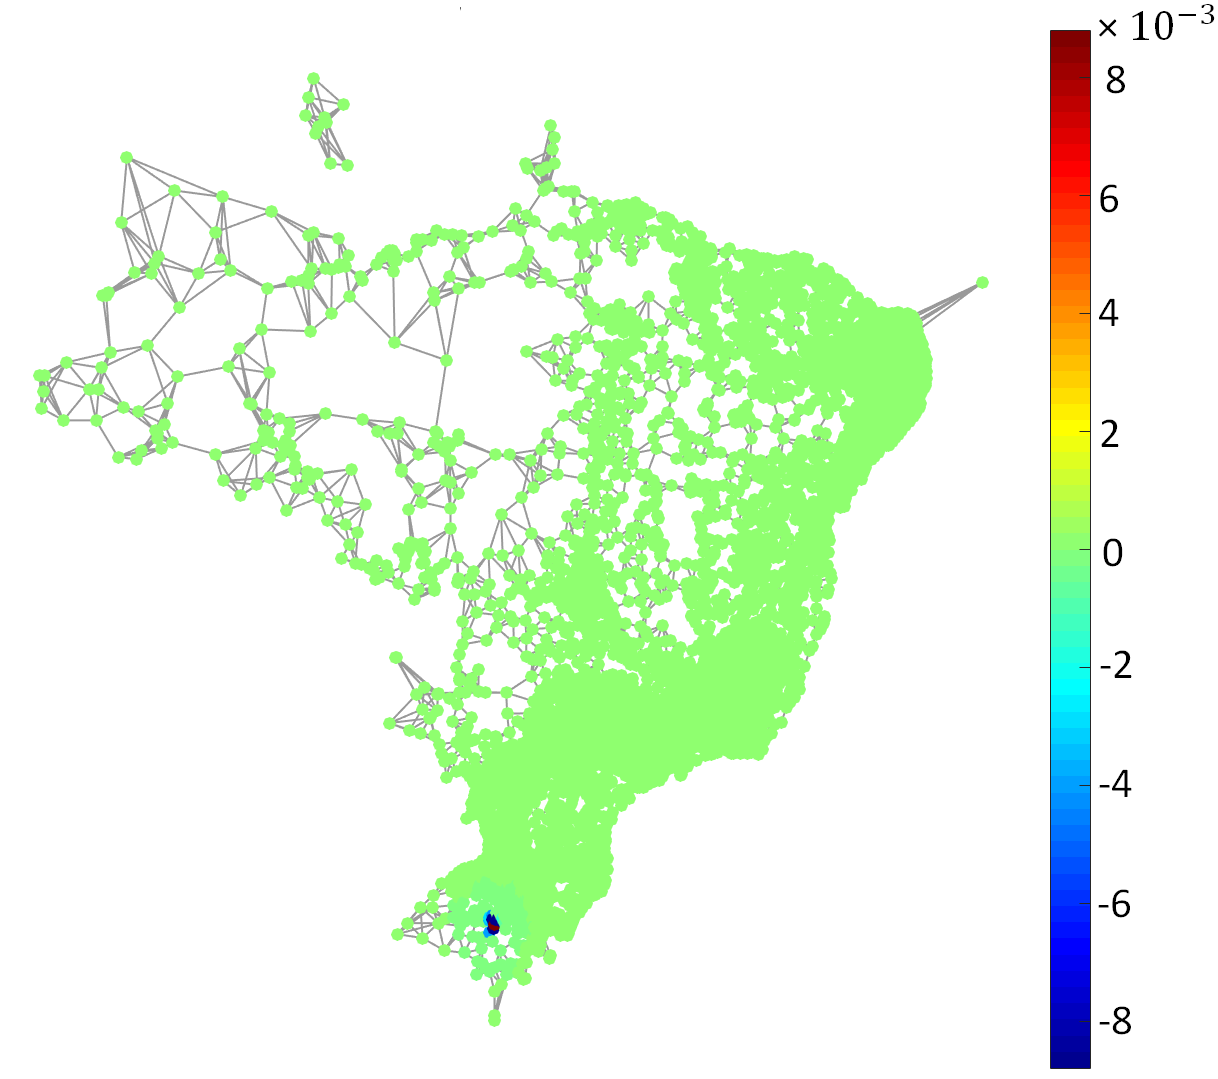
\includegraphics[width=2.8in] {figures/s2.png}
		\label{fig:Brazil_s2}
	}
	\caption{Graph wavelets with center city $v_{83}$. $s_1$ = 1.31, $s_2$ = 0.68.}
	\label{fig:graphwaveletscale}
\end{figure}

\begin{figure}[th]
	\centering
	\subfigure[$W_f(s_1,a)$]{
		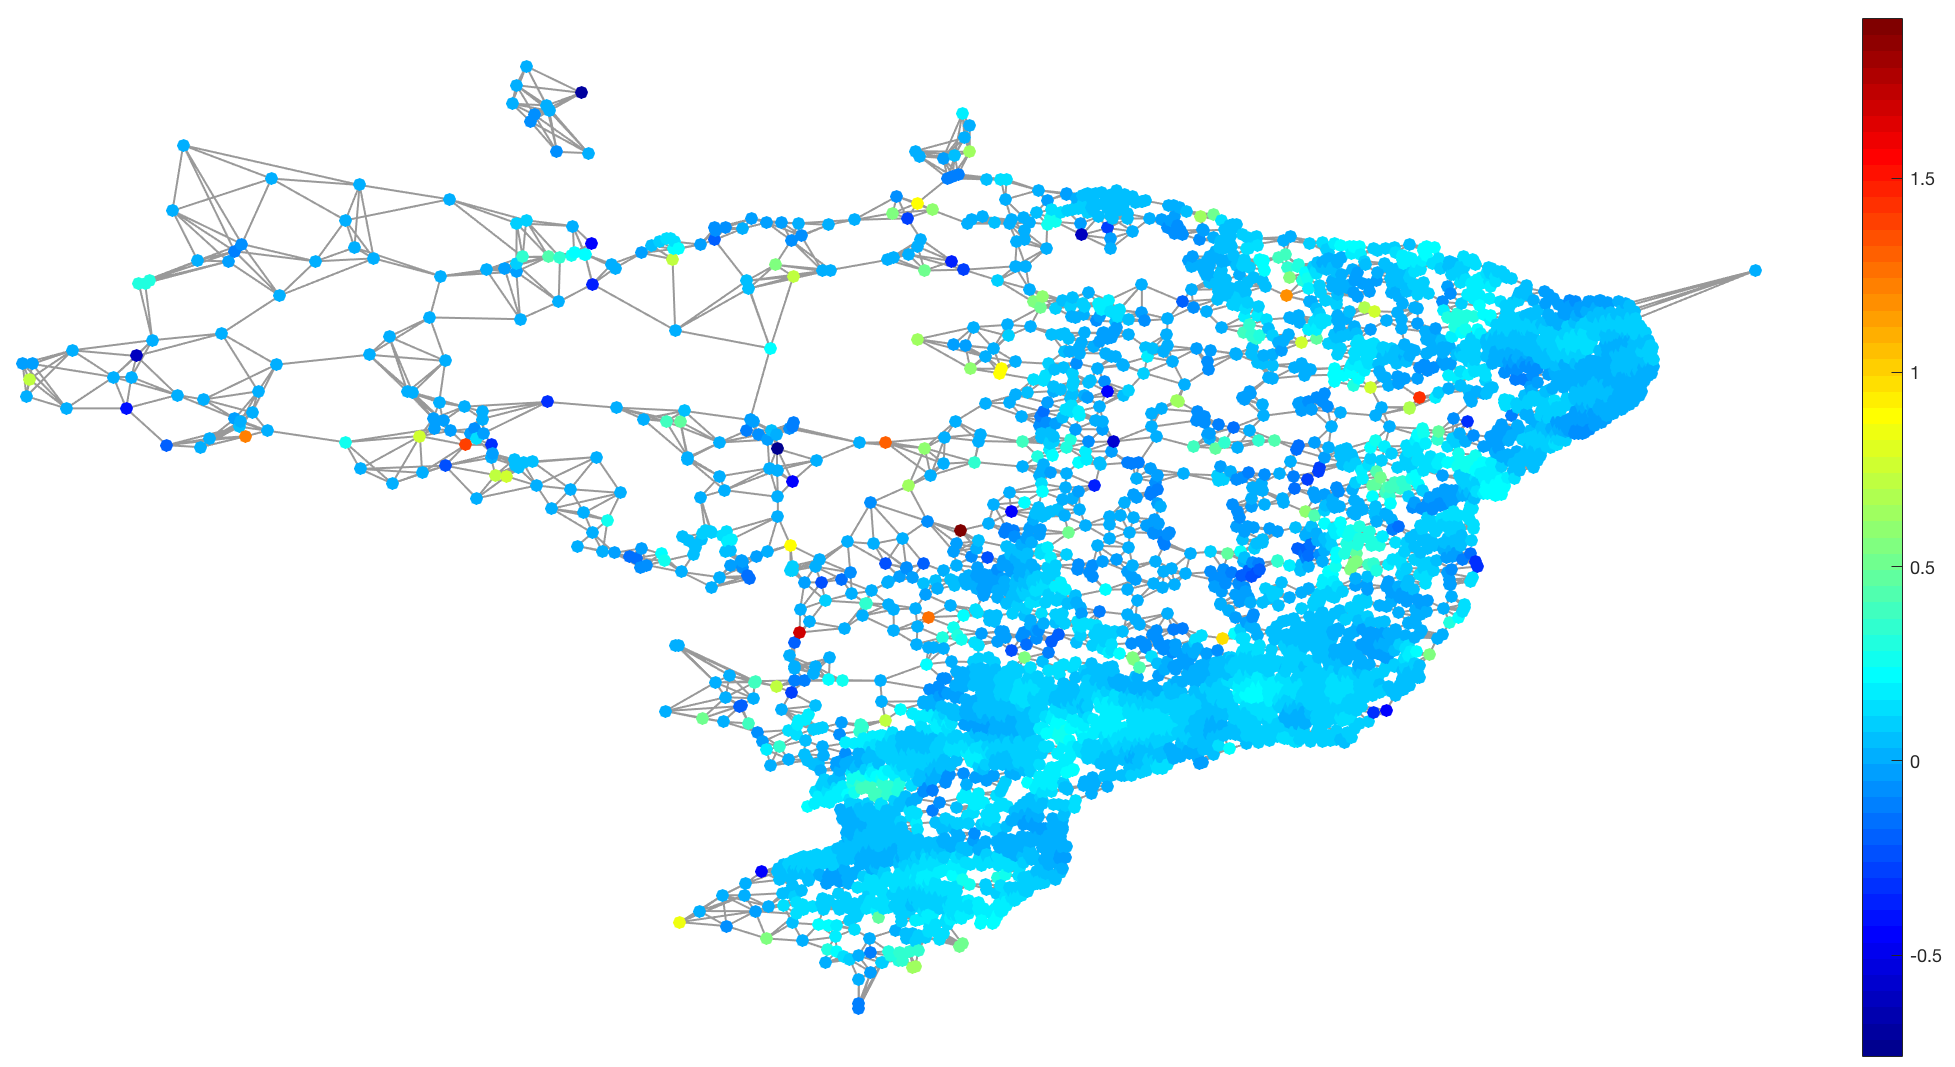
\includegraphics[width=2.4in,height=2.2in] {figures/wavelet_coeff_s1.png}
		\label{fig:Brazil_W_coeff_date31_s3}
	}
	\subfigure[$W_f(s_2,a)$]{
		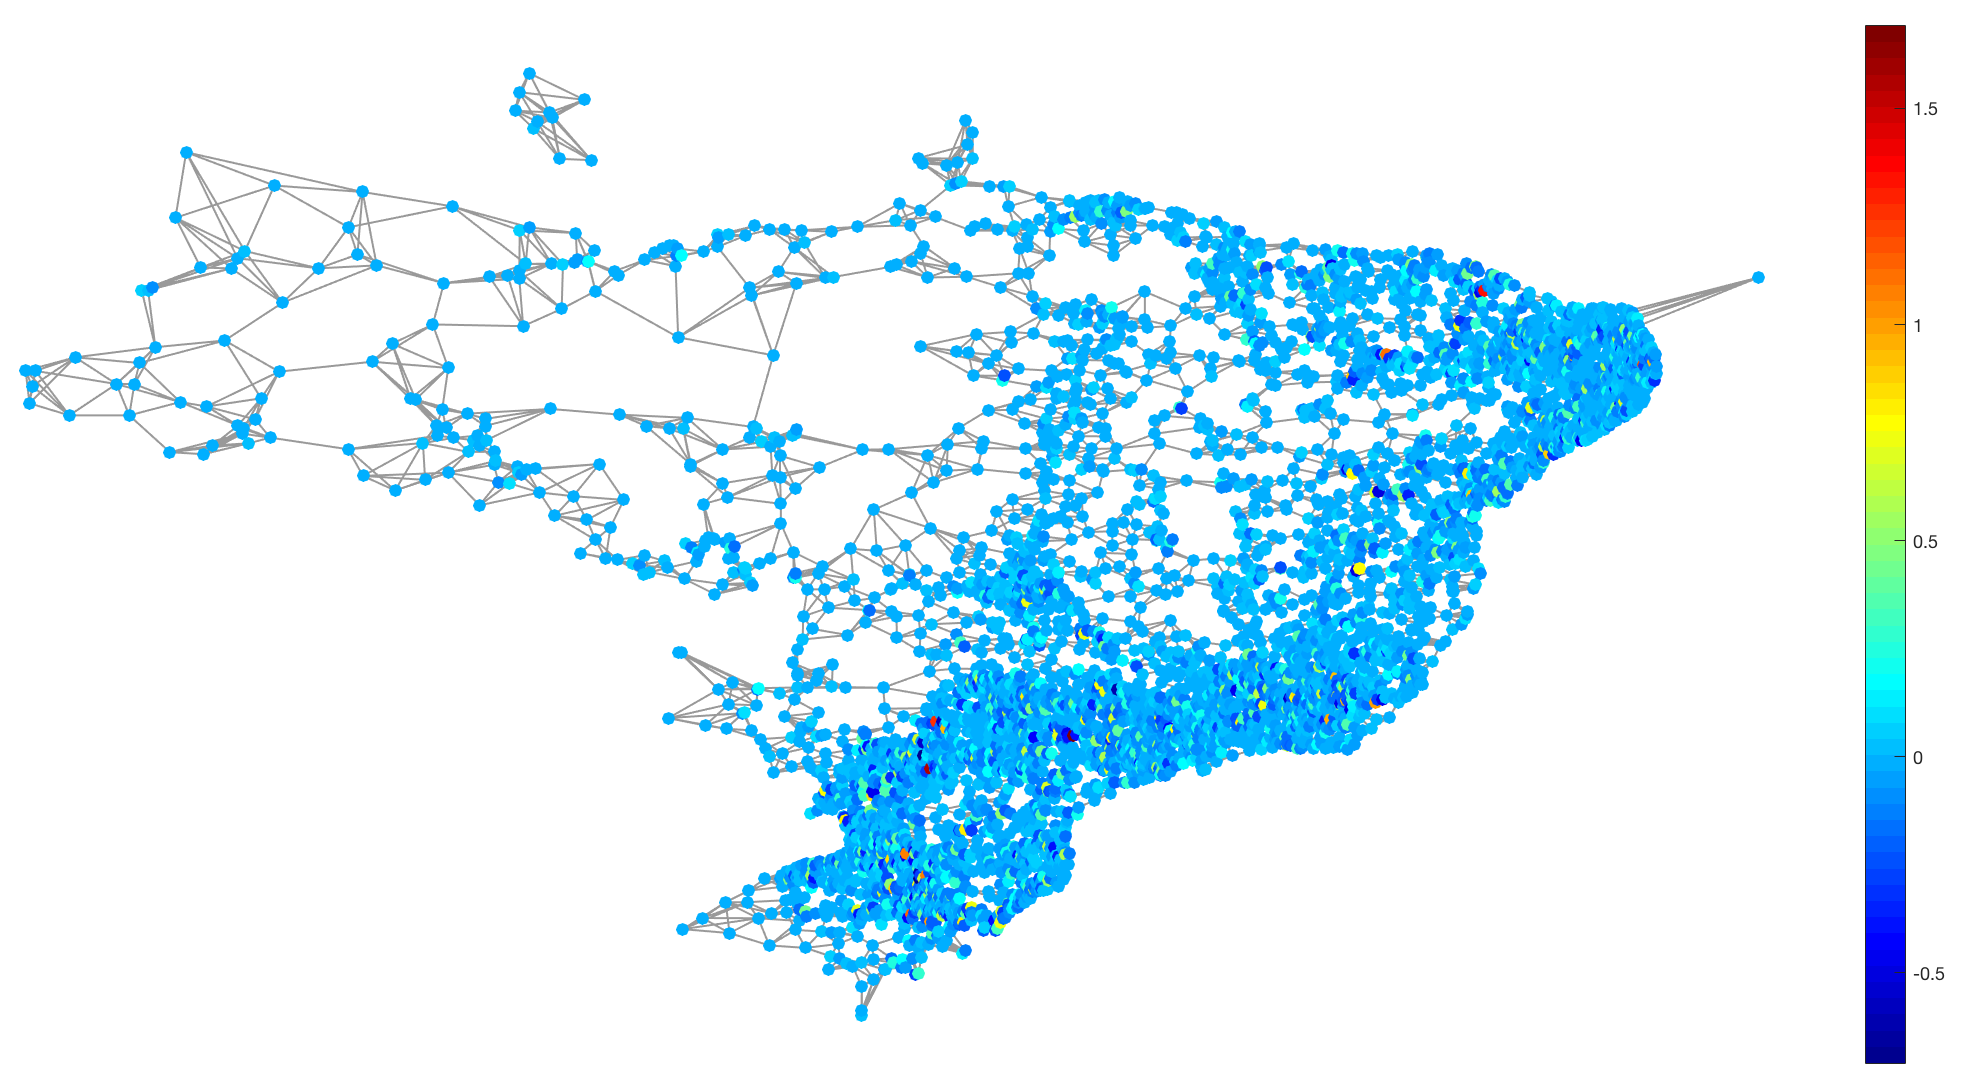
\includegraphics[width=2.4in,height=2.2in] {figures/wavelet_coeff_s6.png}
		\label{fig:Brazil_W_coeff_date31_s5}
	}
	\caption{Graph wavelet coefficient $W_f(s_1,a)$ and $W_f(s_2,a)$.}
	\label{fig:graphwaveletcoefficient}
\end{figure}


\paragraph{Kernel function $g(x)$ and scaling function $h(x)$}
Our choice for the wavelet generating kernel function, $g(x)$, and scaling function $h(x)$ is motivated by our goal to achieve scale-dependent localization. We follow the kernel function setting in~\cite{hammond2011wavelets}, which behaves as a monic power near the origin, and has power law decay for large x, as shown in Figure~\ref{fig:kernel_function}. $g(x)$ and $h(x)$ are set as:
\begin{equation}
g(x) = \left\{ \begin{array}{rl}
 x &\mbox{ for $x<1$} \\
s(x) &\mbox{ for $1\leq x \leq 2$} \\
 2x^{-1} &\mbox{ for $x>2$} \\
       \end{array} \right.
\end{equation} where $s(x)=-5+11x-6x^2+x^3$.
\begin{equation}
h_{x}= 1.385\, exp(-(\frac{20x}{0.6\lambda_{max}})^4)
\end{equation}
The scale set $\{s_j\}_{j=1}^J$ is selected to be equally logarithmically spaced between the minimum and maximum scales $s_1$ and $s_J$, which are defined in~\cite{hammond2011wavelets}. We set $J=6$ in the experiment. Figure~\ref{fig:graphwaveletscale} shows two different scaled wavelets on Brazil's $5$-nearest-neighbor graph. Comparing Figure~\ref{fig:Brazil_s1} with Figure~\ref{fig:Brazil_s2}, we can see that, when scale increases, more cities (with deeper color) are selected. 
Figure~\ref{fig:graphwaveletcoefficient} shows the corresponding wavelet coefficients.
We also try another kernel function, i.e. the Mexican hat function, and find that as long as the kernel function monotonicity is the same,
the differences in wavelet coefficients are negligible.



\paragraph{Anomaly index $\gamma_f(G)$ and $\omega_{th}$}
We claim that the event frequency $\eta$ is linear to $\gamma_f(\mathbf{G})$, described as
\begin{equation}
\label{eq:linear_equation}
\eta = k_0*\gamma_f(\mathbf{G}) + k_1
\end{equation}We use historical data to train $k_0$ and $k_1$ by least square error criterion. Once we know
$k_0$ and $k_1$, given a new $\gamma_f'(\mathbf{G})$, the event number is estimated as $m=\left \lceil \eta' \right \rceil$. Subsequently the
threshold $\omega_{th}$ is set as the $m_{th}$ largest $W_f(s_j,a)$, for all $a\in V$, $0\le j \le J$.


\begin{table}[bt] %!htp
\renewcommand{\arraystretch}{1.1}
\caption{\label{table:models_compare} The performance of graph wavelet vs. baseline and Z-score.}
\scriptsize
\centering
\begin{tabular}{ l | l |l | l | l}
\hline
\textbf{Country} & \textbf{Method}& \textbf{Precision}  & \textbf{Recall}  & \textbf{F-measure} \\
\hline
Brazil & Baseline & 0.052 &0.104 & 0.060\\
       & Z-score & 0.117&0.307 & 0.159 \\
 & Graph wavelet& 0.404 &0.262 & 0.292 \\
\hline
Mexico & Baseline & 0.074 &0.124 & 0.090 \\
       & Z-score & 0.221 &0.147 & 0.168 \\
 & Graph wavelet& 0.397 &0.384 & 0.408 \\
\hline
Venezuela & Baseline & 0.078 &0.053 & 0.059 \\
       & Z-score & 0.197 &0.197 & 0.189 \\
 & Graph wavelet& 0.292 &0.554 & 0.355 \\
\hline
\end{tabular}
\end{table}



\subsection{Performance}
The data for this experiment was gathered for three countries experiencing major protest events, namely Brazil, Mexico and Venezuela, from Jan 2013 to Dec 2014. Taking the Gold Standard Report (GSR)~\cite{ramakrishnan2014beating} as representing ground truth, we applied our new graph wavelet approach as follows. For each day, we determine whether there is any anomaly. If there is, we
identify the group of anomalous cities and compare this set
with the GSR to determine if the selected cities actually experienced protest events on that day and thus show how many of the model's predictions matched the ground truth and how many did not. We use recall, precision, and the F-measure to evaluate the model's performance. To evaluate the effectiveness of our new graph wavelet approach, we also compared the results with those obtained using intuitive approaches such as frequency based random assignment, referred to here as the baseline model, and z-score based selection methods. The baseline model was built according to the historical protest records for each city and thus the model's predictions of the future occurrence of protests were based on frequency. The z-score approach entails
selecting the group of cities whose z-score crosses some threshold, say $|z-score|>3$.



\begin{figure}[h]
	\centering
	\subfigure[Brazil]{
		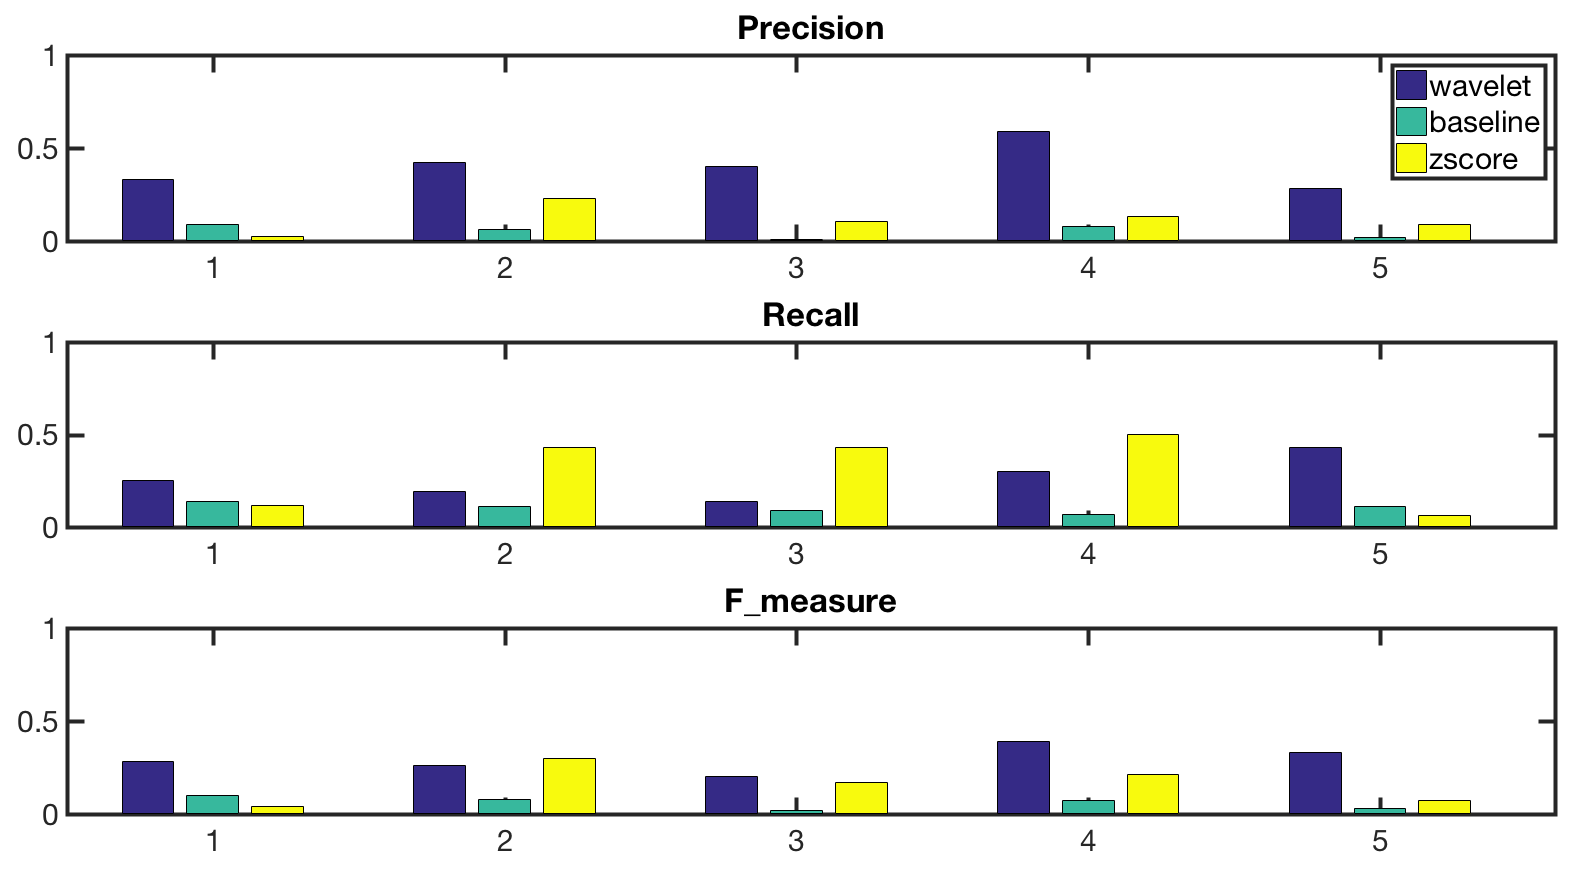
\includegraphics[width= 4.5in, height=1.7in] {figures/performance_compare_bar_graph_brazil.png}
		\label{Brazil_performance}
	}
	\hfill
	\subfigure[Mexico]{
		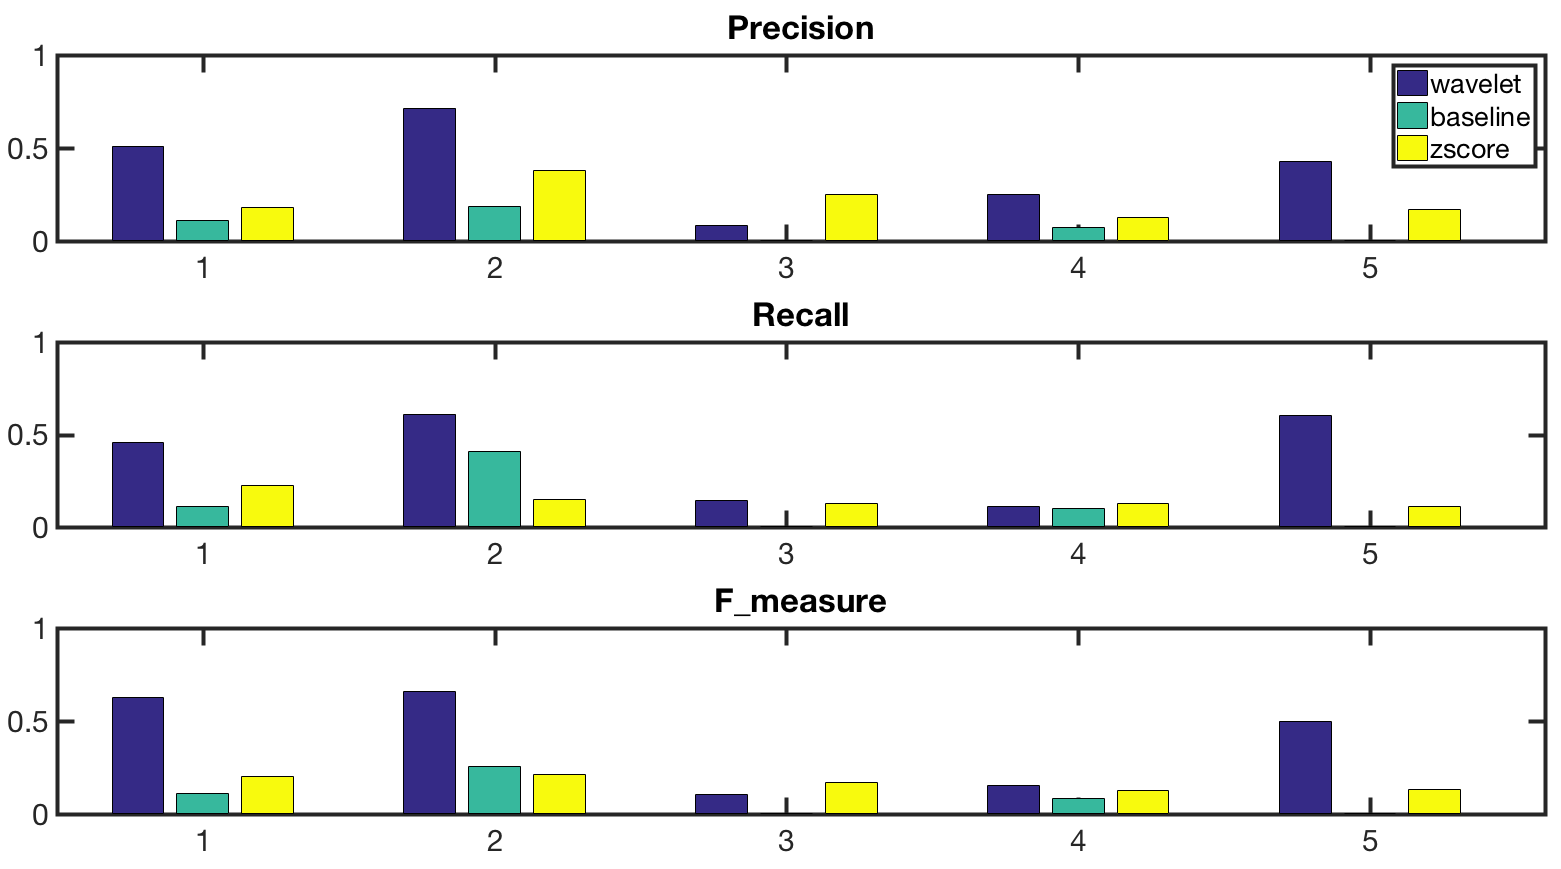
\includegraphics[width= 4.5in, height=1.7in] {figures/performance_compare_bar_graph_mexico.png}
		\label{Mexico_performance}
	}
	\hfill
	\subfigure[Venezuela]{
		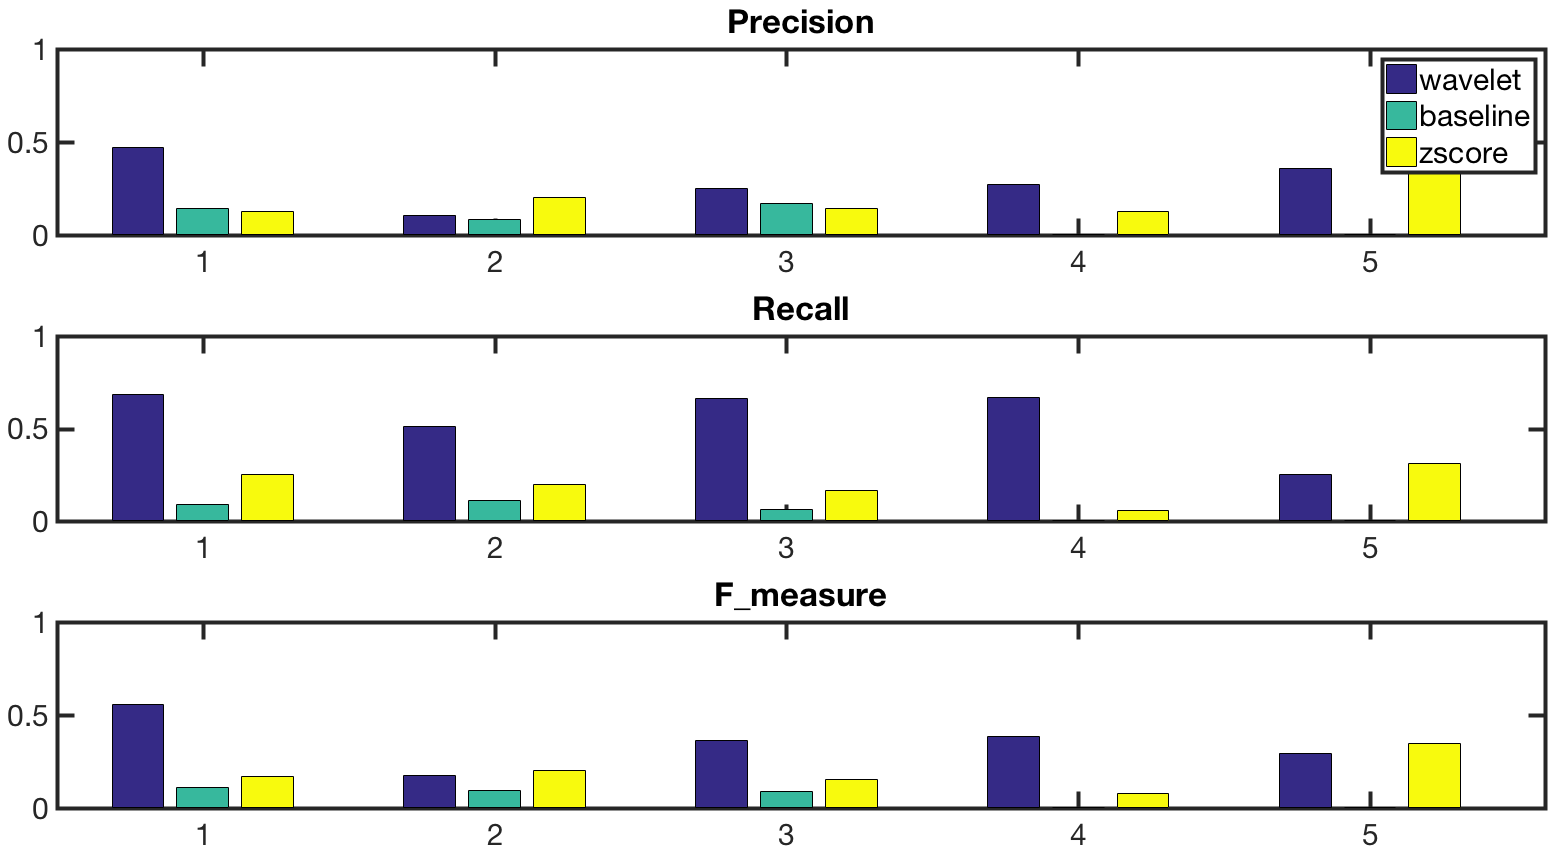
\includegraphics[width= 4.5in, height=1.7in] {figures/performance_compare_bar_graph_venezuela.png}
		\label{Venezuela_performance}
	}
	\caption{Brazil, Mexico and Venezuela protest detection performance.}
\label{fig:threecountry_performance}
\end{figure}


We compared the performance of these three models over the two year test period; the overall results are shown in Table~\ref{table:models_compare}. Generally speaking, the new graph wavelet approach exhibited better precision, recall, and F-measure scores than the baseline model across all three countries. The mean F-measure for the graph wavelet detection across models and countries is greater than that achieved by either of the other prediction models. Interestingly, the graph wavelet approach appears to operate at different efficiency levels for each country. From Figure~\ref{fig:threecountry_performance} we can see that the graph wavelet model has a much higher recall in Venezuela than in Brazil, and an inferior quality of event detection in Mexico compared to Venezuela.



\subsection{Case Studies}
\label{sec:highlighted_results}

\begin{figure}[h]
	\centering
	\subfigure[]{
		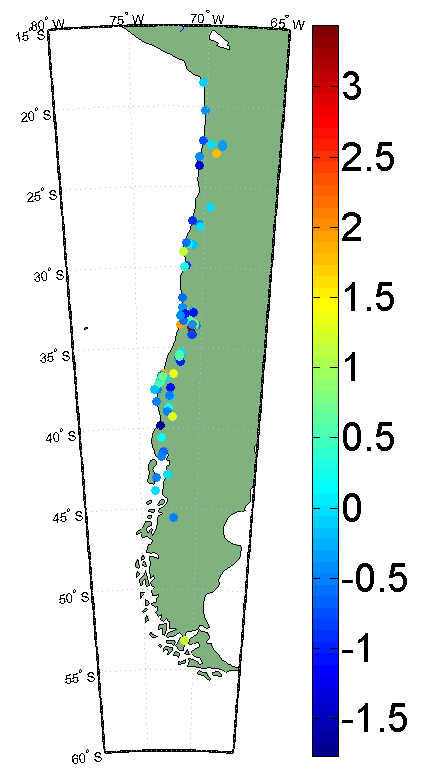
\includegraphics[width=1.4in,height=1.8in] {figures/Chile_absent_zscore_3.png}
		\label{fig:absent_Chile_score}
	}
	\hfill
	\subfigure[]{
		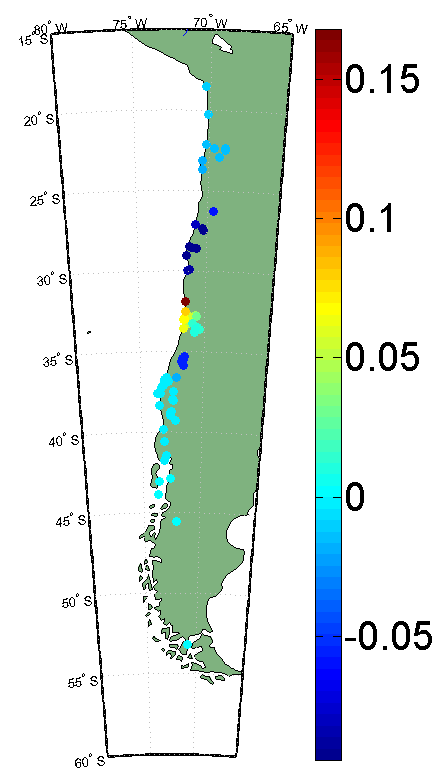
\includegraphics[width=1.4in,height=1.8in] {figures/Chile_absent_wavelet_3.png}
		\label{fig:absent_Chile_wavelet}
	}
	\hfill
	\subfigure[]{
		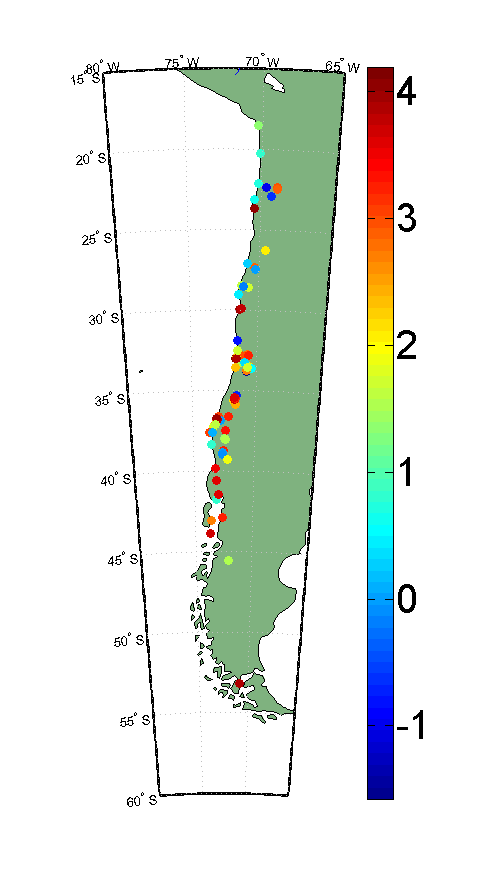
\includegraphics[width=1.4in,height=1.8in] {figures/Chile_burst_zscore_3.png}
		\label{fig:burst_Chile_score}
	}
	\hfill
	\subfigure[]{
		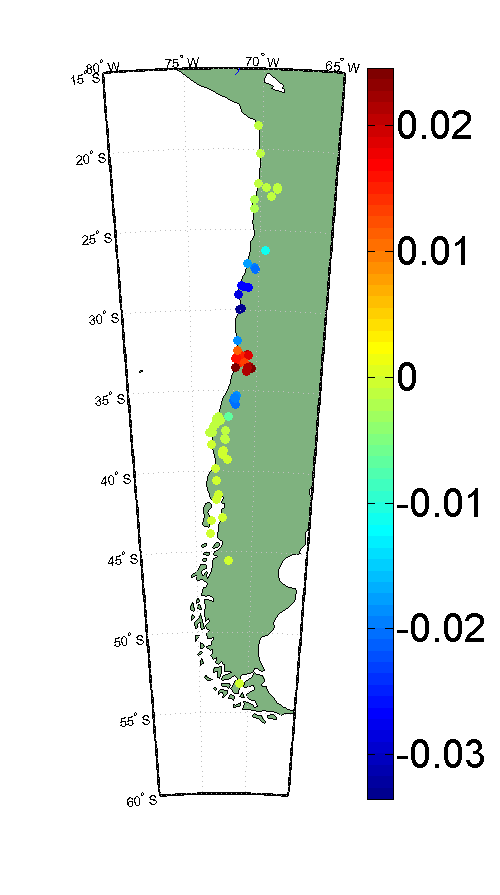
\includegraphics[width=1.4in,height=1.8in] {figures/Chile_burst_wavelet_3.png}
		\label{fig:burst_Chile_wavelet}
	}
	\subfigure[]{
		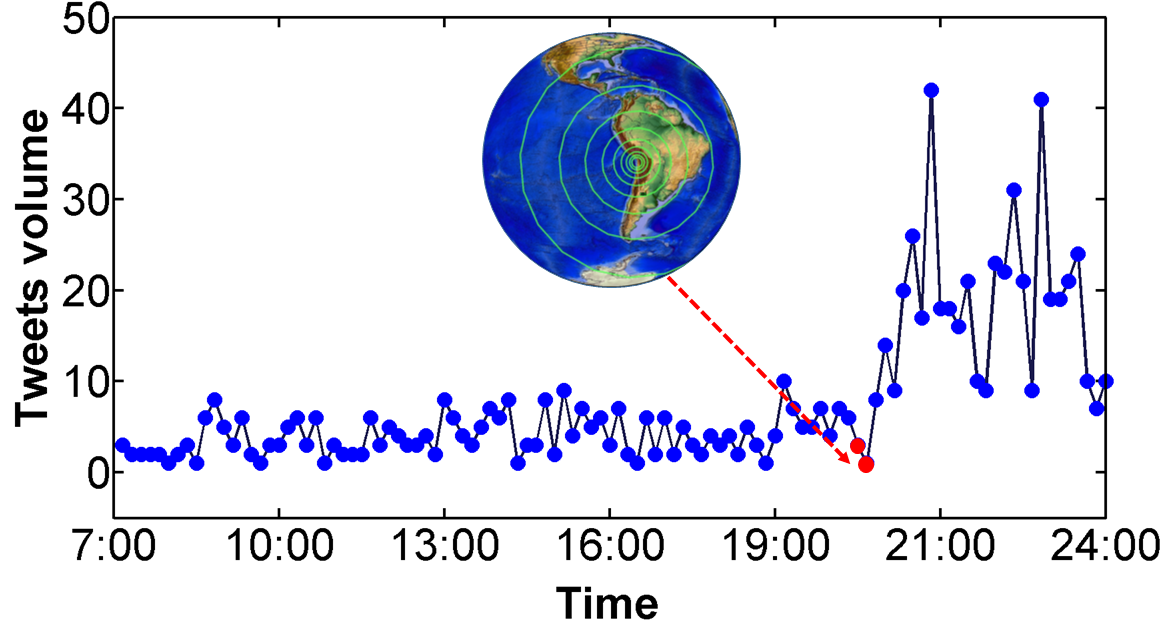
\includegraphics[width=2.8in,height=1.6in] {figures/earthquake_example_10min_circle.png}
		\label{fig:earthquake}
	}
	\subfigure[]{
		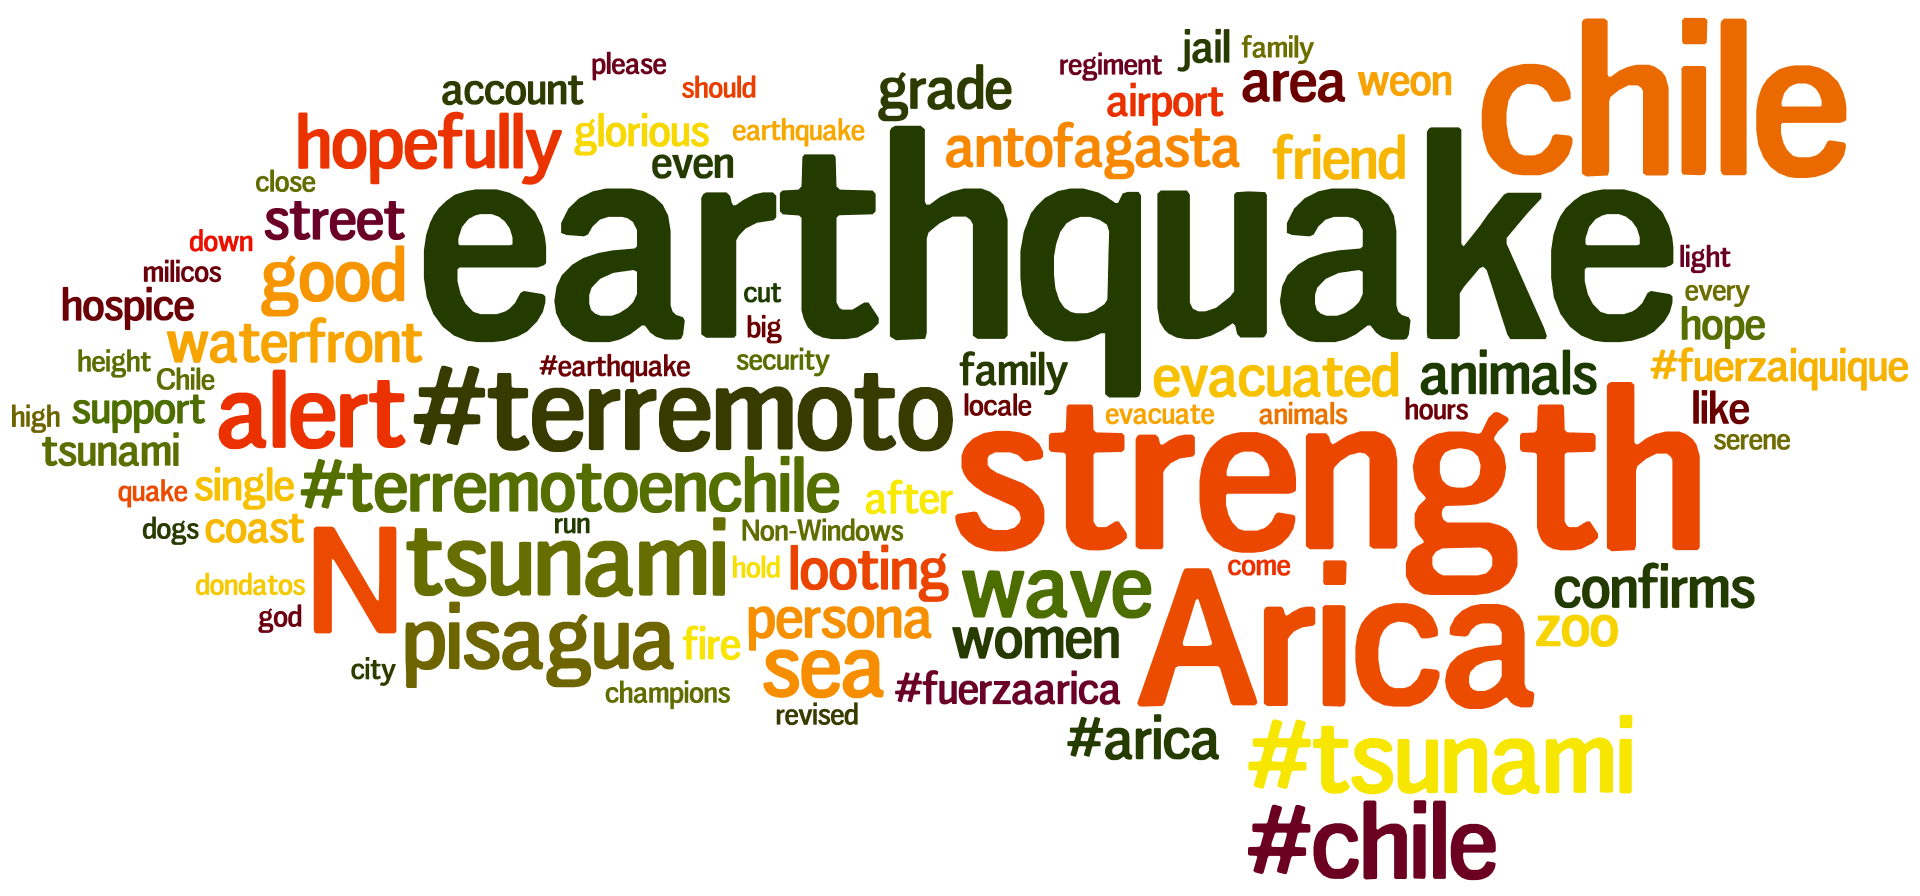
\includegraphics[width=2.8in,height=1.6in] {figures/earthquake_cloud.png}
		\label{fig:earthquake-cloud}
	}
	\caption{Iquique Earthquake, Chile. (a-d) plots show differences in distributions of absenteeism score and wavelet coefficients calculated at 8:45 PM, April 1, 2014 (a-b) involving group absenteeism and later when burst in activity is captured at 11:00 AM, April 2, 2014 (c-d), respectively; (e) Tweet time series for Iquique on April 1, 2014; (f) Word cloud of tweets which mention `Iquique'.}
\label{fig:case1_wavelet}
\end{figure}



\textbf{Case study 1: Iquique Earthquake, Chile.}
On April 1, 2014 at around 8:46 PM (local time) a large earthquake struck off the coast of Chile, northwest of the port city of Iquique. We show the distribution of absenteeism scores and normalized wavelet coefficient values of the graph wavelets from the beginning of this event and throughout the subsequent 24 hours period. As shown in Figure~\ref{fig:absent_Chile_score}, we can clearly see absenteeism behavior, where the scores are dominated by very low (blue spectrum) z-score values (indicating high absenteeism). Likewise, Figure~\ref{fig:absent_Chile_wavelet} depicts low coefficient values for the northern regions of Chile, where the impact of the earthquake was most significant. As the news of earthquake spread throughout the next day, user activity on social media increased. This bursty behavior is clearly visible on April 2nd, at around 11:00 AM. Figure~\ref{fig:burst_Chile_score} shows that the z-scores increase (red spectrum) significantly and the coefficient value distribution (Figure~\ref{fig:burst_Chile_wavelet}) of the graph wavelets for northern regions of Chile are also in the red spectrum. The graph wavelet distributions in Figures~\ref{fig:absent_Chile_wavelet}~\ref{fig:burst_Chile_wavelet} show that the kernel area of the absenteeism/burst wavelets cover most large negative/positive values. In this way, the wavelets identify the abnormal negative/positive groups in absent/burst time intervals, respectively. Furthermore, a high correlation score of 0.726 was calculated for the wavelets from absenteeism and bursty periods of this episode, indicating a strong connection between the burst in activity and the previously observed absenteeism, signaling an event was detected.



\begin{figure}[h]
	\centering
	\subfigure[]{
		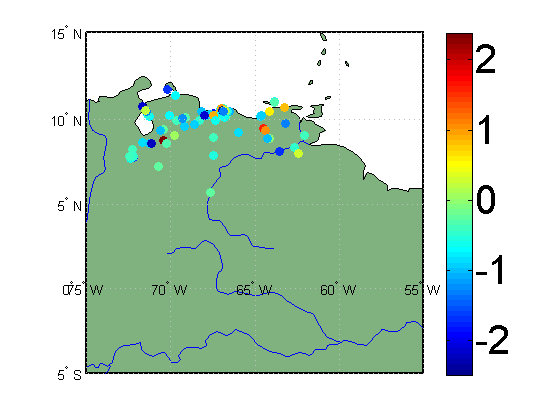
\includegraphics[width=1.4in, height=1.5in] {figures/Venuze_absent_zscore_3.png}
		\label{fig:absent_Venezuela_score}
	}
	\subfigure[]{
		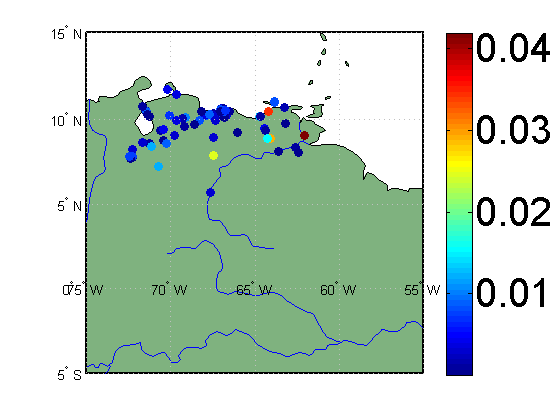
\includegraphics[width=1.4in, height=1.5in] {figures/Venuze_absent_wavelet_3.png}
		\label{fig:absent_Venezuela_wavelet}
	}
	\subfigure[]{
		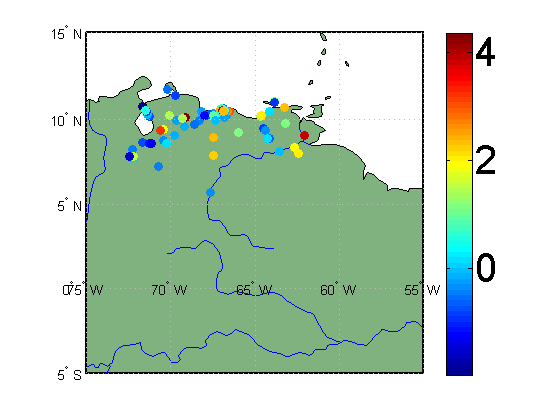
\includegraphics[width=1.4in, height=1.5in] {figures/Venuze_burst_zscore_3.png}
		\label{fig:burst_Venezuela_score}
	}
	\subfigure[]{
		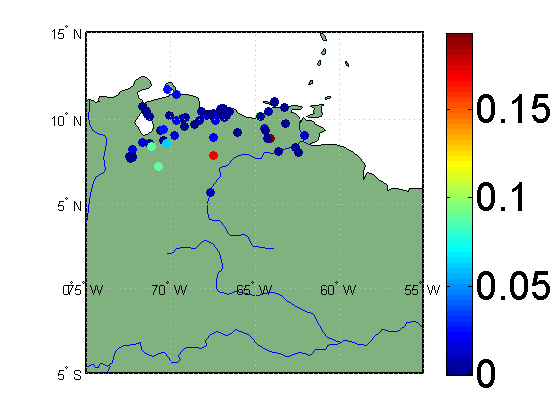
\includegraphics[width=1.4in, height=1.5in] {figures/Venuze_burst_wavelet_3.png}
		\label{fig:burst_Venezuela_wavelet}
	}
	\subfigure[]{
		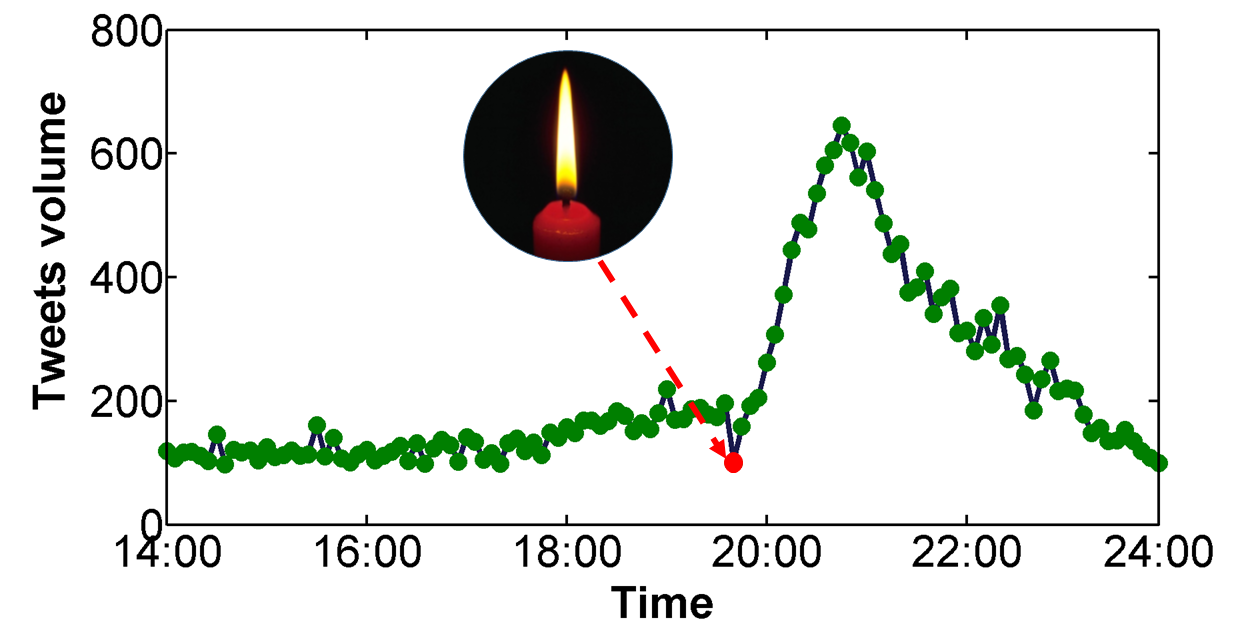
\includegraphics[width=2.8in,height=1.3in] {figures/Veneuela_power_count_all.png}
		\label{fig:power}
	}
	\subfigure[]{
		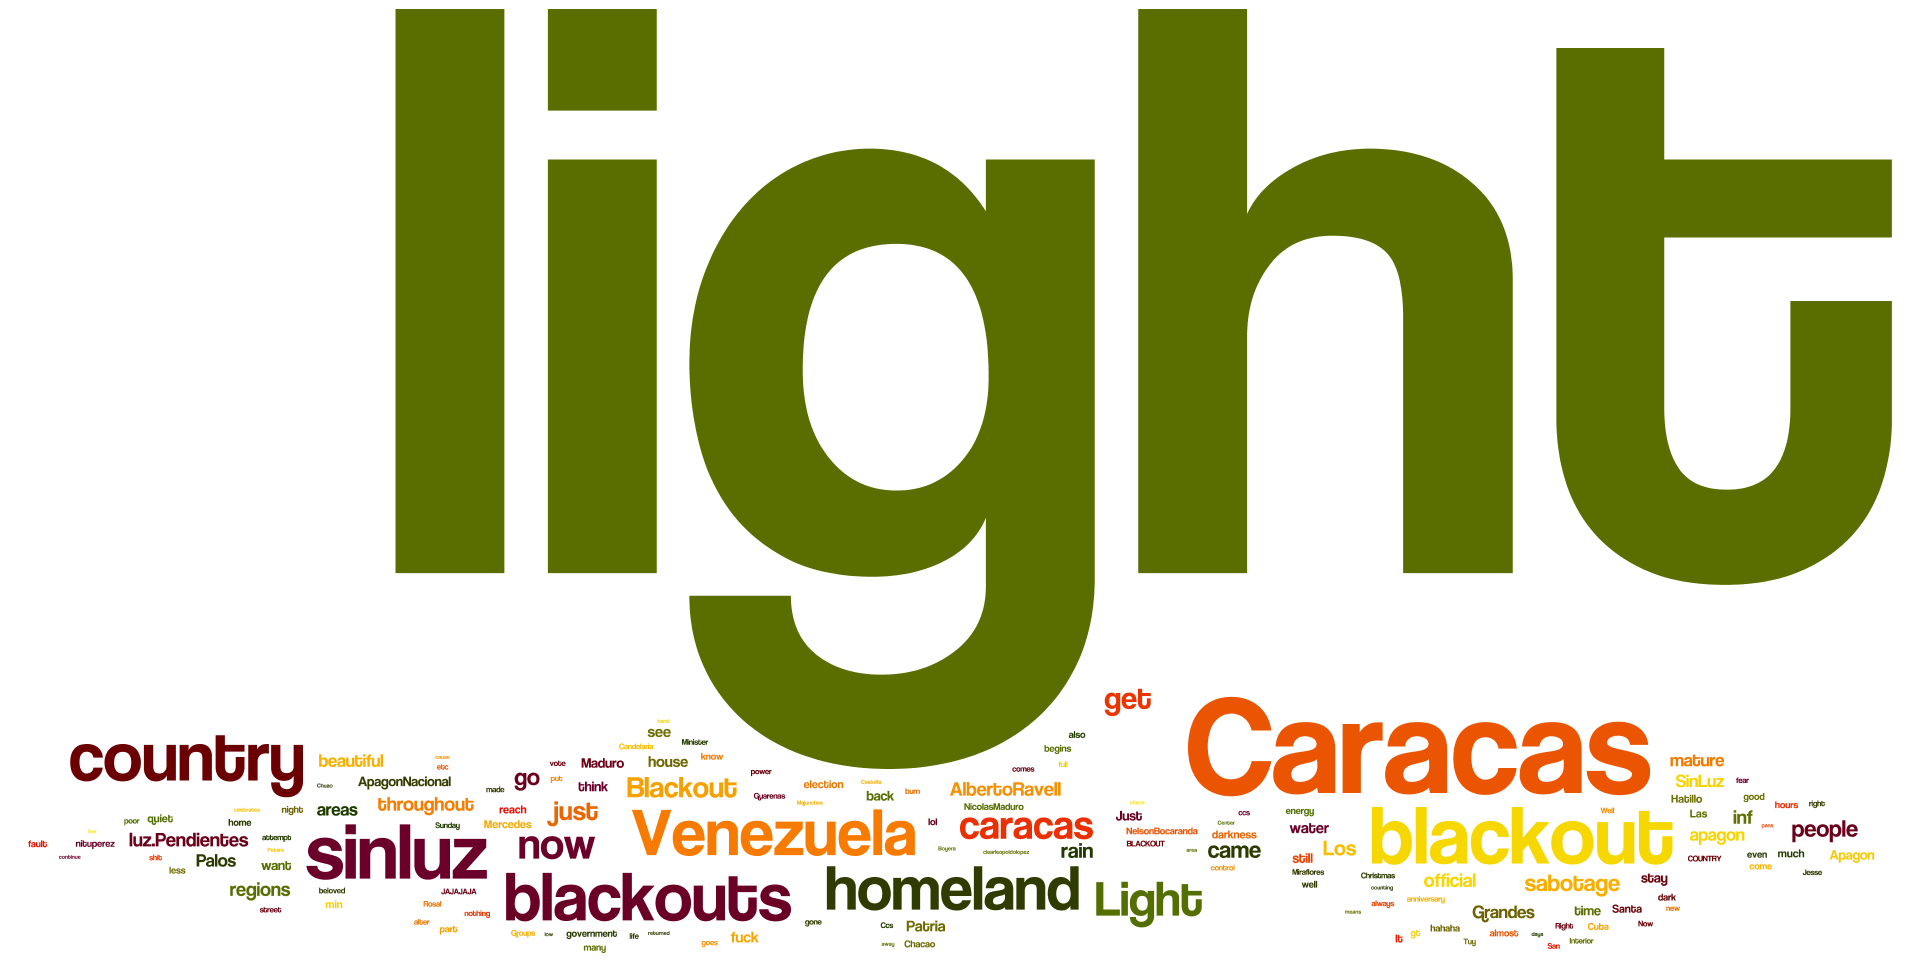
\includegraphics[width=2.8in,height=1.3in] {figures/power-English.png}
		\label{fig:power-cloud}
	}
	\caption{Power Outage in Venezuela. (a-d) plots show differences in distributions of absenteeism score and wavelet coefficients calculated at 7:40 PM, December 2, 2013 (a-b) involving group absenteeism and later when burst in activity is captured at 8:45 PM in the same day (c-d), respectively; (e) Time series of tweets volume on December 2, 2013; (f) Word cloud of tweets mentioning `Caracas'.}
\label{fig:case2_wavelet}
\end{figure}


The graph wavelets generated during the absenteeism time period Figure~\ref{fig:absent_Chile_wavelet} have a central node located in the city of `Iquique'. Looking at the time series (Figure~\ref{fig:earthquake}) of Twitter activity for Iquique and the associated word clouds (Figure~\ref{fig:earthquake-cloud}), we can see how events unfolded during the course of the earthquake. Strong absenteeism is observed from 8:45 PM to 9:20 PM. Examining user mobility via their geotagged tweets from the city of Iquique, on April 1, 2014, the user mobility fraction had increased by 15.4\%.


\textbf{Case Study 2: Massive power outage in Venezuela.}
A massive power outage in Venezuela plunged several major cities, including the capital city Caracas, into darkness around 7:40 PM (local time) on December 2, 2013.
News media reported\footnote{http://www.usatoday.com/story/news/world/2013/12/\hskip0ex 02/\hskip0ex power-failure-caracas-venezuela/3823327/}, that the power outage lasted for 10-15 minutes, and the people of Caracas quickly took to the streets to protest.
This action at the beginning of the episode coincides with the absenteeism period detected by our algorithm.
The scatter plots showing the distribution of absenteeism scores and wavelet coefficients (Figures~\ref{fig:absent_Venezuela_score},~\ref{fig:absent_Venezuela_wavelet}) indicate that most of the low values are less than $0$.
Shortly after the absenteeism, we detected a huge burst in activity around 8:45 PM, signaled by the increased z-scores (low absenteeism) and coefficient values (Figures~\ref{fig:burst_Venezuela_score},~\ref{fig:burst_Venezuela_wavelet}). A correlation score of 0.617 was calculated when comparing the graph wavelets from the absentee and burst periods.


The absenteeism related graph wavelets indicate that the city of Caracas was the central node. Taking a close look at the Twitter volume and tweets from Caracas and surrounding cities, there is a sharp decline in user activity around 7:40 PM and then a huge spike starting at 8:45 PM. The word clouds for the tweet content show a very similar story, with dominant words being `light' and `blackout'; the Spanish phrase `sin luz', which means `no light', became a trending hashtag \#sinluz on Twitter.



\begin{figure}[h]
	\centering
	\subfigure[]{
		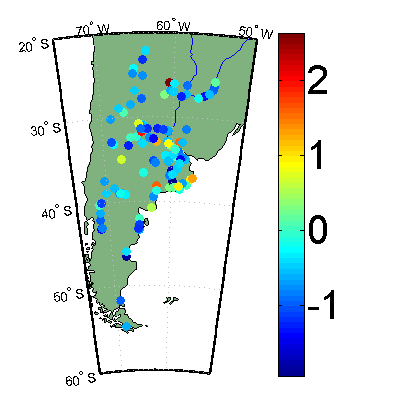
\includegraphics[height=1.5in] {figures/Argentina_absent_zscore_3.png}
		\label{fig:absent_Argentina_score}
	}
	\subfigure[]{
		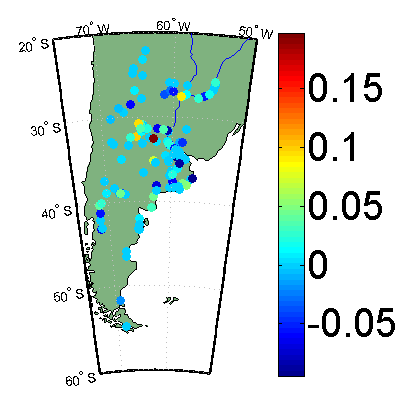
\includegraphics[height=1.5in] {figures/Argentina_absent_wavelet_3.png}
		\label{fig:absent_Argentina_wavelet}
	}
	\subfigure[]{
		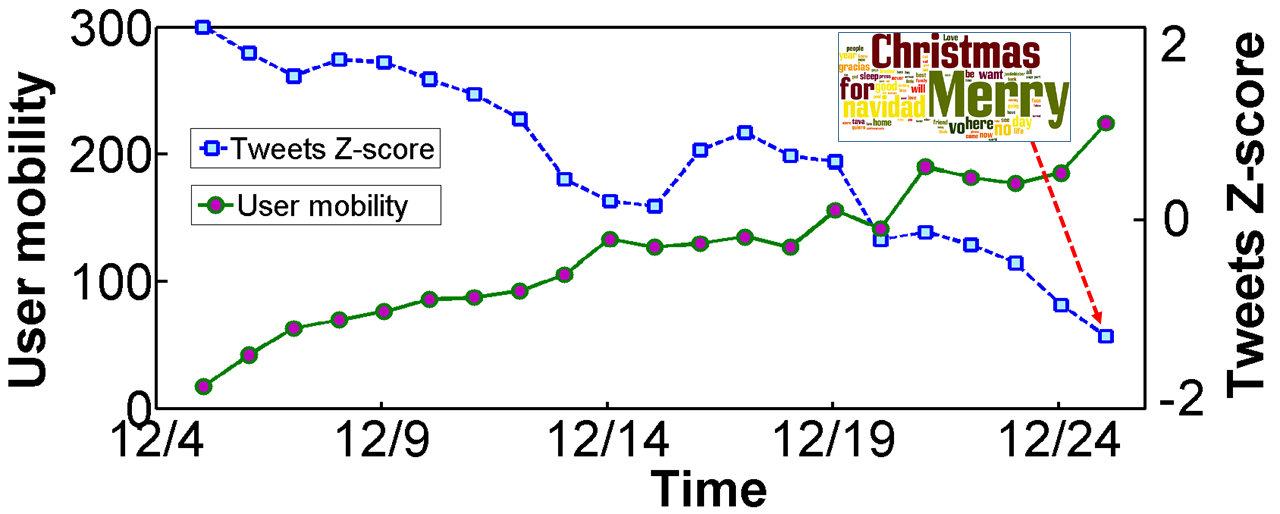
\includegraphics[width=2.6in, height=1.4in] {figures/holiday-cloud.png}
		\label{fig:holiday-cloud}
	}
	\caption{The Christmas Day in Argentina: (a-b) plots show distributions of (a) absenteeism score and (b) wavelet coefficients calculated on December 25, 2013; (c) Time series comparing absenteeism score and user mobility corresponding to tweets between December 5 - 25, 2013.}
\label{fig:case3_wavelet}
\end{figure}


\textbf{Case Study 3: Christmas Day.}
As noted earlier, absenteeism behavior may not always lead to a spike in activity. For example, our model detected strong absenteeism in social media activity for major holidays such as Christmas Day that was not followed by a bursty period in Twitter activity. This is likely because people tend to travel to visit family during the holidays. This is supported by low values of z-scores or high absenteeism in Figure~\ref{fig:absent_Argentina_score} and wavelet coefficients in Figure~\ref{fig:absent_Argentina_wavelet} with respect to Argentinian tweets on December 25, 2013. Hence, no subsequent burst period was detected for this event. Interestingly as Christmas Day approached, Figure~\ref{fig:holiday-cloud} shows that user mobility gradually increases and the z-score decreases, signaling greater absenteeism. We used Pearson's correlation coefficient to measure the two time series and found a correlation score of -0.94.





%%%%%%%%%%%%%%%%%%%%%%%%%%%% end %%%%%%%%%%%%%%%%%%%%%%%%%
%\begin{table*}[th] %!htp
% \renewcommand{\arraystretch}{1}
% \caption{\label{table:list_events} Selected major events in South America countries}
% \scriptsize
% \centering
% \begin{tabular}{ p{0.5cm}| p{2cm} | p{2.2cm} | p{2.2cm} | p{2.2cm} | p{2.5cm} | p{3cm} }
%  \hline
%  \textbf{No.} & \textbf{Events}& \textbf{ Absenteeism } & \textbf{Response time} & \textbf{Correlation}&\textbf{Central location} \\ [1ex]
%  \hline
%        1& Earthquake & 8:45 PM & 3 hours & 0.73 &Iquique, Chile\\
%        2& Blackout & 7:40 PM & 1 hour & 0.81& Caracas, Venezuela \\
%        3& holiday & one day & 2 days & 0.33 & \\        \hline
% \end{tabular}
%\end{table*}


%Public holidays are typical events causing group absenteeism. One of the most dominant reason is, during public holidays, especially long-time holiday, people tend to travel, which resulting in a high level of local user mobility, and users' mobility will cause Twitter absenteeism accordingly.
%We calculating more cases Pearson's correlation, and plot their distribution in Figure~\ref{fig:pearson}, of which the median value of correlation score is -0.88, and the average correlation score is -0.79. We can see the user mobility plays a forceful role in influencing Twitter absenteeism.

%\subsection{Performance}
%We use the data set on February 27, 2014, and set the time window as one day. We plot the comparison results from two aspects:  running time complexity, and parameter sensibility in figure~\ref{fig:performance},~\ref{fig:running_time},~\ref{fig:sensibility}.
%\begin{figure}[ht]
%	\centering
%	\subfigure[matrix]{
%		\includegraphics[width=1.55in,height=1in] {figures/performance1.png}
%		\label{fig:performance1}
%	}
%	\subfigure[graph]{
%		\includegraphics[width=1.55in,height=1in] {figures/performance2.png}
%		\label{fig:performance2}
%	}
%	\caption{running time vs input parameter.}
%	\label{fig:performance}
%\end{figure}
%\paragraph{Running time}From Figure~\ref{fig:performance}, we can see that the running time of minimal matrix approach increases extremely fast when $A$ is larger than 0.09. While in graph wavelet approach, the increasing speed is much stable as $d_{th}$ increases. This is because minimal matrix approach's time complexity is in proportion to $A^2$, while graph wavelet approach's time complexity is proportional to $d_{th}$. From Figure~\ref{fig:running_time}, we can see clearly that for the minimal matrix algorithm, the running time complexity also increase sharply with the input size $n$, while in graph wavelet approach, the increase speed is moderate. This is because the minimal matrix approach's timing complexity is $O(N^3)$, while graph wavelet approach's time complexity is $O(N^2)$. Thus, the graph wavelet approach is better  than minimal matrix approach in term of running time for a larger absenteeism group.
%\begin{figure}[h]
%	\centering
%	\subfigure[matrix]{
%		\includegraphics[width=1.55in,height=1in] {figures/running_time1.png}
%		\label{fig:running1}
%	}
%	\subfigure[graph]{
%		\includegraphics[width=1.55in,height=1in] {figures/running_time2.png}
%		\label{fig:running2}
%	}
%	\caption{Running time vs input size.}
%	\label{fig:running_time}
%\end{figure}
%\paragraph{Parameter sensibility}In minimal matrix approach, set the input parameter as $A$, and the optimal absenteeism group as $P_{min}$. When $A$ is changed to $A$', the optimal absenteeism group is changed to $P_{min}$, define the output error as the city number that exists in $P_{min}$ but not in $P_{min}'$, and denoted as $P_{min}-P_{min}'$. We define the parameter sensibility as: $$sensibility=\frac{{|P_{min}-P_{min}'|}/{|P_{min}|}}{|A-A'|/{A}}.$$ We plot the minimal matrix approach and graph wavelet approach's sensibility in Figure~\ref{fig:sensibility}. In the minimal matrix approach, when the input parameter error is smaller than 20\%, the output absenteeism group error is less than 5\%. While in the graph wavelet approach, the output absenteeism group error is linear to the input error parameter. This is probably because minimal matrix approach aggregates all the absenteeism score covered by the region, and usually has a much larger city number than the graph wavelet approach, and makes minimal matrix approach better at anti-noise.  All in all, the minimal matrix algorithm focuses on all the cities in the cover group, and has a better global performance at anti-noise, while is inferior to the graph wavelet counterpart in term of running time complexity.
%\begin{figure}[h]
%	\centering
%	\subfigure[matrix]{
%		\includegraphics[width=1.55in,height=1in] {figures/sensibility1.png}
%		\label{fig:sensibility1}
%	}
%	\subfigure[graph]{
%		\includegraphics[width=1.55in,height=1in] {figures/sensibility2.png}
%		\label{fig:sensibility2}
%	}
%	\caption{Sensibility comparison of the two algorithms.}
%	\label{fig:sensibility}
%\end{figure}




% % % % % % % % % % % % % the end% % % % % % % %
%
%\begin{figure}[ht]
%	\centering
%	\subfigure[]{
%		\includegraphics[width=1.55in,height=1in] {figures/Curitiba-Brazil1-cloud.png}
%		\label{fig:holiday}
%	}
%	\subfigure[]{
%		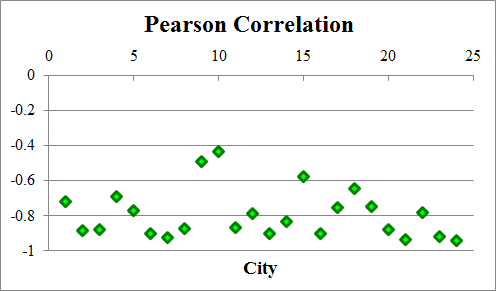
\includegraphics[width=1.55in,height=1in] {figures/pearson1.png}
%		\label{fig:pearson}
%	}
%	\caption{(a) User mobility time series and corresponding absenteeism score, from Dec 5, 2013 to Dec 25, 2013. (b) Pearson correlation score distribution of user mobility and absenteeism score.}
%\label{fig:case3}
%\end{figure}

%Now we show experimental results of our algorithm on highlighted case studies (see Table~\ref{table:list_events}):
%
%\begin{table*}[th] %!htp
%	\renewcommand{\arraystretch}{1}
%	\caption{\label{table:list_events} Selected major events in South America countries}
%	\scriptsize
%	\centering
%	\begin{tabular}{ p{0.5cm}| p{1.5cm} | p{8cm} | p{1.5cm}}
%		\hline
%		\textbf{No.} & \textbf{Date}& \textbf{ Events} & \textbf{Test Areas}   \\ [1ex]
%		\hline
%        1& 2013-06-17 & Brazilian Spring: Protests in over 100 cities, over 2 million people & Brazil  \\		
%        2& 2013-12-02 & Power cut leaves much of Venezuela without electricity & Venezuela \\
%        3& 2013-12-24 & Floods, more than 50,000 people are forced to flee their homes & Brazil\\
%        4& 2013-12-25 & Christmas holiday  & Argentina \\
%        5& 2013-12-30 & Power supply disrupted in heatwave in Buenos Aires, Argentina & Argentina \\
%        6& 2014-04-01 &  M8.2 earthquake struck off the coast of Chile, epicenter is Iquique & Chile  \\
%        7 & 2014-05-21 & Bus strike paralyzes Brazil's biggest city as World Cup looms & Brazil \\			\hline
%	\end{tabular}
%\end{table*}


%The wavelet scales $t_j$ are selected to be logarithmically equispaced between the minimum and maximum scales $t_J$ and $t_1$, with the upper bound $\lambda_{max}$ of the spectrum of $L$. The placement of the maximum scales $t_1$ as well as the scaling function kernel $h$ will be determined by the selection of $\lambda_{min}=\frac{\lambda_{min}}{K}$, where $K$ is a design parameter of the transformation. We then set $t_1$ so that $g(t_1x)$ has power-law decay for $x>\lambda_{min}$, and set $t_J$ so that $g(t_Jx)$ provides monotonicity of the polynomial for $x < \lambda_{max}$. This is achieved by $t_1=\frac{x_2}{\lambda_{min}}$, and $t_J=\frac{x_2}{\lambda_{max}}$. For the scaling function kernel we take $h(x)=\gamma exp(-({{\frac{x}{\lambda_{min}}}})^4)$, where $\gamma$ is set such that $h(0)$ has the same value as the maximum value of $g$.
%
%At each time point the graph has an Z-score vector $f$ and when we get the lowest value for function $< \psi_{t,n},f>$ the corresponding wavelet $\psi_{t,n}$ is reported as an absenteeism pattern.

